\section{Question 8.5}

\subsection{Question}
Generate the mean average precision, recall-precision graph, average NDCG at 5 and 10, and precision at 10 for the entire CACM query set.

\subsection{Approach}
The \texttt{getrel.py} and \texttt{q85.py} scripts were used to complete this question. They can be found in Listings \ref{listing:getrel} and \ref{listing:q85}.

\subsection{Results}

Using only the queries for which relevance judgments exist the mean average precision, NDCG @5 and 10, and the precision @ 10 were calculated.  The results can be found in Table \ref{tab:q85}.

\begin{table}[h!]
\centering
\begin{tabular}{ | c | c | c | c | }
\hline
MAP & NDCG @5 & NDCG @10 & Prec. @10 \\
\hline
0.339552098123 & 0.461648777763 & 0.381724764912 & 0.317647058824 \\
\hline
\end{tabular}
\caption{Calculations for all CACM queries from all retrieved documents.}
\label{tab:q85}
\end{table}

The generated recall-precision graph for the entire query set can be found in Figure \ref{fig:overallavg}.

\begin{figure}[H]
\centering
\label{fig:overallavg}
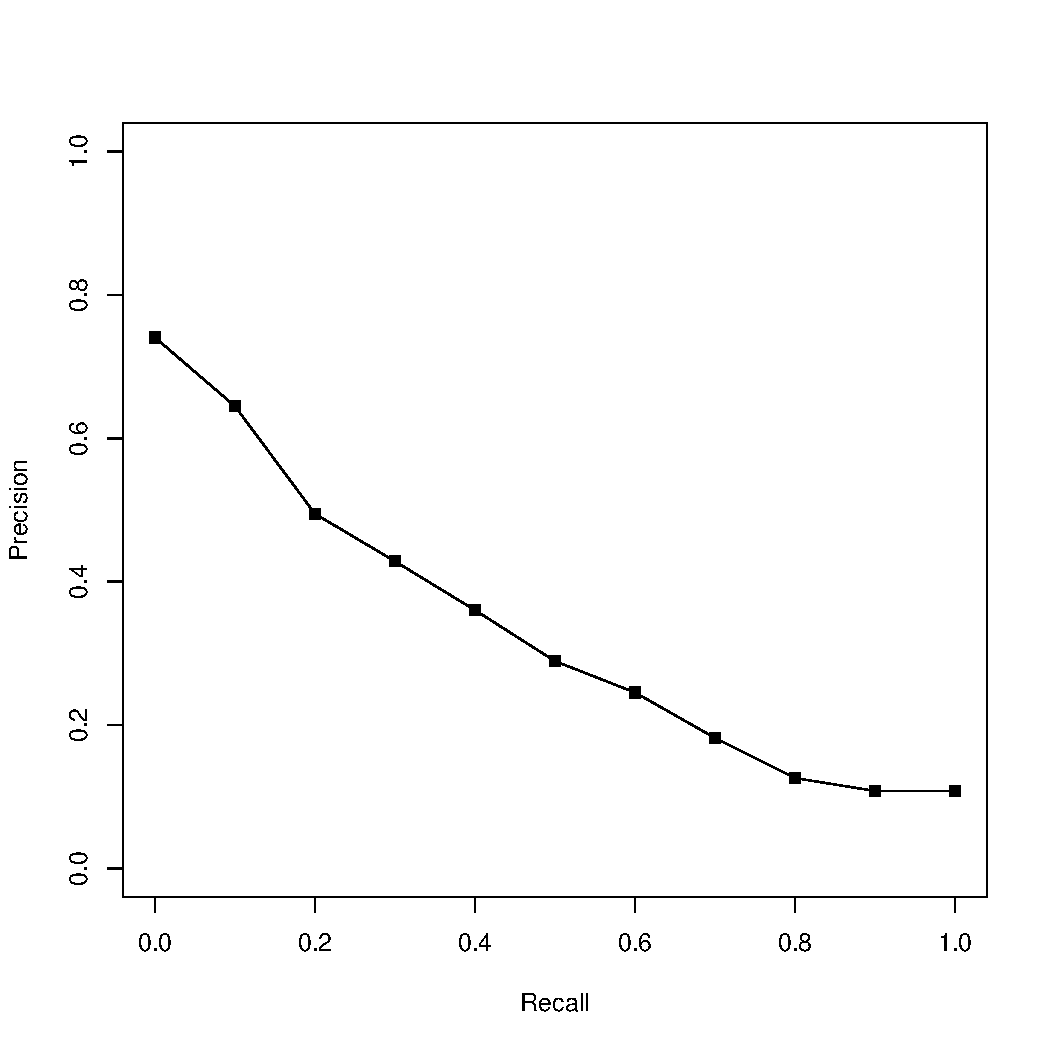
\includegraphics[scale=.6]{code/getrel/avgq85.pdf}
\caption{Recall-precision graph for all CACM Queries.}
\end{figure}
